% Options for packages loaded elsewhere
\PassOptionsToPackage{unicode}{hyperref}
\PassOptionsToPackage{hyphens}{url}
%
\documentclass[
  twocolumn]{article}
\usepackage{amsmath,amssymb}
\usepackage{lmodern}
\usepackage{iftex}
\ifPDFTeX
  \usepackage[T1]{fontenc}
  \usepackage[utf8]{inputenc}
  \usepackage{textcomp} % provide euro and other symbols
\else % if luatex or xetex
  \usepackage{unicode-math}
  \defaultfontfeatures{Scale=MatchLowercase}
  \defaultfontfeatures[\rmfamily]{Ligatures=TeX,Scale=1}
  \setmainfont[]{Verdana}
\fi
% Use upquote if available, for straight quotes in verbatim environments
\IfFileExists{upquote.sty}{\usepackage{upquote}}{}
\IfFileExists{microtype.sty}{% use microtype if available
  \usepackage[]{microtype}
  \UseMicrotypeSet[protrusion]{basicmath} % disable protrusion for tt fonts
}{}
\makeatletter
\@ifundefined{KOMAClassName}{% if non-KOMA class
  \IfFileExists{parskip.sty}{%
    \usepackage{parskip}
  }{% else
    \setlength{\parindent}{0pt}
    \setlength{\parskip}{6pt plus 2pt minus 1pt}}
}{% if KOMA class
  \KOMAoptions{parskip=half}}
\makeatother
\usepackage{xcolor}
\IfFileExists{xurl.sty}{\usepackage{xurl}}{} % add URL line breaks if available
\IfFileExists{bookmark.sty}{\usepackage{bookmark}}{\usepackage{hyperref}}
\hypersetup{
  pdftitle={Formatting, Latex, plot and table samples},
  pdfauthor={Fabian Koch},
  hidelinks,
  pdfcreator={LaTeX via pandoc}}
\urlstyle{same} % disable monospaced font for URLs
\usepackage{color}
\usepackage{fancyvrb}
\newcommand{\VerbBar}{|}
\newcommand{\VERB}{\Verb[commandchars=\\\{\}]}
\DefineVerbatimEnvironment{Highlighting}{Verbatim}{commandchars=\\\{\}}
% Add ',fontsize=\small' for more characters per line
\usepackage{framed}
\definecolor{shadecolor}{RGB}{248,248,248}
\newenvironment{Shaded}{\begin{snugshade}}{\end{snugshade}}
\newcommand{\AlertTok}[1]{\textcolor[rgb]{0.94,0.16,0.16}{#1}}
\newcommand{\AnnotationTok}[1]{\textcolor[rgb]{0.56,0.35,0.01}{\textbf{\textit{#1}}}}
\newcommand{\AttributeTok}[1]{\textcolor[rgb]{0.77,0.63,0.00}{#1}}
\newcommand{\BaseNTok}[1]{\textcolor[rgb]{0.00,0.00,0.81}{#1}}
\newcommand{\BuiltInTok}[1]{#1}
\newcommand{\CharTok}[1]{\textcolor[rgb]{0.31,0.60,0.02}{#1}}
\newcommand{\CommentTok}[1]{\textcolor[rgb]{0.56,0.35,0.01}{\textit{#1}}}
\newcommand{\CommentVarTok}[1]{\textcolor[rgb]{0.56,0.35,0.01}{\textbf{\textit{#1}}}}
\newcommand{\ConstantTok}[1]{\textcolor[rgb]{0.00,0.00,0.00}{#1}}
\newcommand{\ControlFlowTok}[1]{\textcolor[rgb]{0.13,0.29,0.53}{\textbf{#1}}}
\newcommand{\DataTypeTok}[1]{\textcolor[rgb]{0.13,0.29,0.53}{#1}}
\newcommand{\DecValTok}[1]{\textcolor[rgb]{0.00,0.00,0.81}{#1}}
\newcommand{\DocumentationTok}[1]{\textcolor[rgb]{0.56,0.35,0.01}{\textbf{\textit{#1}}}}
\newcommand{\ErrorTok}[1]{\textcolor[rgb]{0.64,0.00,0.00}{\textbf{#1}}}
\newcommand{\ExtensionTok}[1]{#1}
\newcommand{\FloatTok}[1]{\textcolor[rgb]{0.00,0.00,0.81}{#1}}
\newcommand{\FunctionTok}[1]{\textcolor[rgb]{0.00,0.00,0.00}{#1}}
\newcommand{\ImportTok}[1]{#1}
\newcommand{\InformationTok}[1]{\textcolor[rgb]{0.56,0.35,0.01}{\textbf{\textit{#1}}}}
\newcommand{\KeywordTok}[1]{\textcolor[rgb]{0.13,0.29,0.53}{\textbf{#1}}}
\newcommand{\NormalTok}[1]{#1}
\newcommand{\OperatorTok}[1]{\textcolor[rgb]{0.81,0.36,0.00}{\textbf{#1}}}
\newcommand{\OtherTok}[1]{\textcolor[rgb]{0.56,0.35,0.01}{#1}}
\newcommand{\PreprocessorTok}[1]{\textcolor[rgb]{0.56,0.35,0.01}{\textit{#1}}}
\newcommand{\RegionMarkerTok}[1]{#1}
\newcommand{\SpecialCharTok}[1]{\textcolor[rgb]{0.00,0.00,0.00}{#1}}
\newcommand{\SpecialStringTok}[1]{\textcolor[rgb]{0.31,0.60,0.02}{#1}}
\newcommand{\StringTok}[1]{\textcolor[rgb]{0.31,0.60,0.02}{#1}}
\newcommand{\VariableTok}[1]{\textcolor[rgb]{0.00,0.00,0.00}{#1}}
\newcommand{\VerbatimStringTok}[1]{\textcolor[rgb]{0.31,0.60,0.02}{#1}}
\newcommand{\WarningTok}[1]{\textcolor[rgb]{0.56,0.35,0.01}{\textbf{\textit{#1}}}}
\usepackage{graphicx}
\makeatletter
\def\maxwidth{\ifdim\Gin@nat@width>\linewidth\linewidth\else\Gin@nat@width\fi}
\def\maxheight{\ifdim\Gin@nat@height>\textheight\textheight\else\Gin@nat@height\fi}
\makeatother
% Scale images if necessary, so that they will not overflow the page
% margins by default, and it is still possible to overwrite the defaults
% using explicit options in \includegraphics[width, height, ...]{}
\setkeys{Gin}{width=\maxwidth,height=\maxheight,keepaspectratio}
% Set default figure placement to htbp
\makeatletter
\def\fps@figure{htbp}
\makeatother
\setlength{\emergencystretch}{3em} % prevent overfull lines
\providecommand{\tightlist}{%
  \setlength{\itemsep}{0pt}\setlength{\parskip}{0pt}}
\setcounter{secnumdepth}{-\maxdimen} % remove section numbering
\usepackage{booktabs}
\usepackage{longtable}
\usepackage{array}
\usepackage{multirow}
\usepackage{wrapfig}
\usepackage{float}
\usepackage{colortbl}
\usepackage{pdflscape}
\usepackage{tabu}
\usepackage{threeparttable}
\usepackage{threeparttablex}
\usepackage[normalem]{ulem}
\usepackage{makecell}
\usepackage{xcolor}
\ifLuaTeX
  \usepackage{selnolig}  % disable illegal ligatures
\fi

\title{Formatting, Latex, plot and table samples}
\usepackage{etoolbox}
\makeatletter
\providecommand{\subtitle}[1]{% add subtitle to \maketitle
  \apptocmd{\@title}{\par {\large #1 \par}}{}{}
}
\makeatother
\subtitle{output: Rmarkdown PDF}
\author{Fabian Koch}
\date{}

\begin{document}
\maketitle

\onecolumn

\begin{Shaded}
\begin{Highlighting}[]
\KeywordTok{library}\NormalTok{(tidyverse) }\CommentTok{# import/wrangle}
\end{Highlighting}
\end{Shaded}

\begin{verbatim}
## -- Attaching packages --------------------------------------- tidyverse 1.3.0 --
\end{verbatim}

\begin{verbatim}
## v ggplot2 3.3.3     v purrr   0.3.4
## v tibble  3.0.4     v dplyr   1.0.2
## v tidyr   1.1.2     v stringr 1.4.0
## v readr   1.4.0     v forcats 0.5.0
\end{verbatim}

\begin{verbatim}
## -- Conflicts ------------------------------------------ tidyverse_conflicts() --
## x dplyr::filter() masks stats::filter()
## x dplyr::lag()    masks stats::lag()
\end{verbatim}

\begin{Shaded}
\begin{Highlighting}[]
\KeywordTok{library}\NormalTok{(ggplot2) }\CommentTok{# plot/maps}
\KeywordTok{library}\NormalTok{(tmap) }\CommentTok{# Dataset/Maps}
\KeywordTok{library}\NormalTok{(kableExtra) }\CommentTok{# tables}
\end{Highlighting}
\end{Shaded}

\begin{verbatim}
## 
## Attaching package: 'kableExtra'
\end{verbatim}

\begin{verbatim}
## The following object is masked from 'package:dplyr':
## 
##     group_rows
\end{verbatim}

\begin{Shaded}
\begin{Highlighting}[]
\KeywordTok{library}\NormalTok{(viridis) }\CommentTok{# palettes}
\end{Highlighting}
\end{Shaded}

\begin{verbatim}
## Loading required package: viridisLite
\end{verbatim}

\twocolumn

\hypertarget{muxf6gliche-packages}{%
\subsubsection{Mögliche Packages}\label{muxf6gliche-packages}}

\href{https://github.com/rstudio/rticles}{rtcles}

Mögliche Lösungen für 2 Spalten:
\url{https://github.com/yihui/rmarkdown-cookbook/issues/19}

\hypertarget{text}{%
\subsubsection{Text}\label{text}}

\hypertarget{headline-1}{%
\section{Headline 1}\label{headline-1}}

\hypertarget{headline-2}{%
\subsection{Headline 2}\label{headline-2}}

\hypertarget{headline-3}{%
\subsubsection{Headline 3}\label{headline-3}}

\hypertarget{headline-4}{%
\paragraph{Headline 4}\label{headline-4}}

\hypertarget{headline-5}{%
\subparagraph{Headline 5}\label{headline-5}}

Lorem ipsum dolor sit amet, consetetur sadipscing elitr, sed diam nonumy
eirmod tempor invidunt ut labore et dolore magna aliquyam erat, sed diam
voluptua. At vero eos et accusam et justo duo dolores et ea rebum. Stet
clita kasd gubergren, no sea takimata sanctus est Lorem ipsum dolor sit
amet. Lorem ipsum dolor sit amet, consetetur sadipscing elitr, sed diam
nonumy eirmod tempor invidunt ut labore et dolore magna aliquyam erat,
sed diam voluptua.

vero eos et accusam et justo duo dolores et ea rebum. Stet clita kasd
gubergren, no sea takimata sanctus est Lorem ipsum dolor sit amet.Lorem
ipsum dolor sit amet, consetetur sadipscing elitr, sed diam nonumy
eirmod tempor invidunt ut labore et dolore magna aliquyam erat, sed diam
voluptua. At vero eos et accusam et justo duo dolores et ea rebum. Stet
clita kasd gubergren, no sea takimata sanctus est Lorem ipsum dolor sit
amet. Lorem ipsum dolor sit amet, consetetur sadipscing elitr, sed diam
nonumy eirmod tempor invidunt ut labore et dolore magna aliquyam erat,
sed diam voluptua. At vero eos et accusam et justo duo dolores et ea
rebum. Stet clita kasd gubergren, no sea takimata sanctus est Lorem
ipsum dolor sit amet.

Lorem ipsum dolor sit amet, consetetur sadipscing elitr, sed diam nonumy
eirmod tempor invidunt ut labore et dolore magna aliquyam erat, sed diam
voluptua. At vero eos et accusam et justo duo dolores et ea rebum. Stet
clita kasd gubergren, no sea takimata sanctus est Lorem ipsum dolor sit
amet. Lorem ipsum dolor sit amet, consetetur sadipscing elitr, sed diam
nonumy eirmod tempor invidunt ut labore et dolore magna aliquyam erat,
sed diam voluptua. At vero eos et accusam et justo duo dolores et ea
rebum. Stet clita kasd gubergren, no sea takimata sanctus est Lorem
ipsum dolor sit amet.Lorem ipsum dolor sit amet, consetetur sadipscing
elitr, sed diam nonumy eirmod tempor invidunt ut labore et dolore magna
aliquyam erat, sed diam voluptua. At vero eos et accusam et justo duo
dolores et ea rebum. Stet clita kasd gubergren, no sea takimata sanctus
est Lorem ipsum dolor sit amet. Lorem ipsum dolor sit amet, consetetur
sadipscing elitr, sed diam nonumy eirmod tempor invidunt ut labore et
dolore magna aliquyam erat, sed diam voluptua. At vero eos et accusam et
justo duo dolores et ea rebum. Stet clita kasd gubergren, no sea
takimata sanctus est Lorem ipsum dolor sit amet.

\onecolumn

\hypertarget{data}{%
\subsubsection{Data}\label{data}}

\begin{Shaded}
\begin{Highlighting}[]
\KeywordTok{data}\NormalTok{(}\StringTok{"World"}\NormalTok{)}

\CommentTok{# Data mit geometry}
\NormalTok{WorldGeom <-}\StringTok{ }\NormalTok{World}
\CommentTok{# Data ohne}
\NormalTok{WorldData <-}\StringTok{ }\NormalTok{World }\OperatorTok\StringTok{ }
\StringTok{  }\NormalTok{sf}\OperatorTok{::}\KeywordTok{st_drop_geometry}\NormalTok{()}
\end{Highlighting}
\end{Shaded}

\hypertarget{map}{%
\subsubsection{Map}\label{map}}

Lorem ipsum dolor sit amet, consetetur sadipscing elitr, sed diam nonumy
eirmod tempor invidunt ut labore et dolore magna aliquyam erat, sed diam
voluptua. At vero eos et accusam et justo duo dolores et ea rebum. Stet
clita kasd gubergren, no sea takimata sanctus est Lorem ipsum dolor sit
amet. Lorem ipsum dolor sit amet, consetetur sadipscing elitr, sed diam
nonumy eirmod tempor invidunt ut labore et dolore magna aliquyam erat,
sed diam voluptua. At vero eos et accusam et justo duo dolores et ea
rebum. Stet clita kasd gubergren, no sea takimata sanctus est Lorem
ipsum dolor sit amet.

\begin{Shaded}
\begin{Highlighting}[]
\CommentTok{# Data }
\NormalTok{mapData <-}\StringTok{ }\NormalTok{WorldGeom }\OperatorTok\StringTok{ }
\StringTok{  }\KeywordTok{select}\NormalTok{(}
\NormalTok{    name,}
\NormalTok{    continent,}
\NormalTok{    pop_est,}
\NormalTok{    income_grp,}
\NormalTok{    geometry) }\OperatorTok\StringTok{ }
\StringTok{  }\KeywordTok{filter}\NormalTok{(continent }\OperatorTok{==}\StringTok{ "Asia"}\NormalTok{) }\OperatorTok\StringTok{ }
\StringTok{  }\KeywordTok{mutate}\NormalTok{(}
    \CommentTok{# Vereinigung der 5 Kategorien zu 3}
    \DataTypeTok{income_grp =}\NormalTok{ forcats}\OperatorTok{::}\KeywordTok{fct_collapse}\NormalTok{(income_grp,}
      \DataTypeTok{Hoch =} \KeywordTok{c}\NormalTok{(}\StringTok{"1. High income: OECD"}\NormalTok{, }\StringTok{"2. High income: nonOECD"}\NormalTok{),}
      \DataTypeTok{Mittel =} \KeywordTok{c}\NormalTok{(}\StringTok{"3. Upper middle income"}\NormalTok{, }\StringTok{"4. Lower middle income"}\NormalTok{),}
      \DataTypeTok{Niedrig =} \KeywordTok{c}\NormalTok{(}\StringTok{"5. Low income"}\NormalTok{)))}





\CommentTok{# Plot}
\NormalTok{map <-}\StringTok{  }\KeywordTok{ggplot}\NormalTok{() }\OperatorTok{+}
\StringTok{    }\KeywordTok{geom_sf}\NormalTok{(}
      \DataTypeTok{data =}\NormalTok{ mapData, }
      \KeywordTok{aes}\NormalTok{(}\DataTypeTok{fill =}\NormalTok{ income_grp)) }\OperatorTok{+}
\StringTok{    }\CommentTok{# Externe Farbpalette, Beispiel viridis}
\StringTok{    }\CommentTok{# https://www.rdocumentation.org/packages/viridis/versions/0.5.1/topics/scale_color_viridis}
\StringTok{    }\NormalTok{viridis}\OperatorTok{::}\KeywordTok{scale_fill_viridis}\NormalTok{(}
      \CommentTok{# Diskrete Variable (Einkommensgruppen)}
      \DataTypeTok{discrete =} \OtherTok{TRUE}\NormalTok{,}
      \CommentTok{# Umkehr der Palette, damit dunkel = low income}
      \DataTypeTok{direction =} \DecValTok{-1}\NormalTok{) }\OperatorTok{+}
\StringTok{    }\KeywordTok{labs}\NormalTok{(}
      \DataTypeTok{title =} \StringTok{"Titel"}\NormalTok{,}
      \DataTypeTok{subtitle =} \StringTok{"Untertitel"}\NormalTok{,}
      \DataTypeTok{caption =} \StringTok{"Fußnote"}\NormalTok{,}
      \DataTypeTok{tag =} \StringTok{"label"}\NormalTok{,}
      \DataTypeTok{fill =} \StringTok{"Titel Legende"}\NormalTok{) }\OperatorTok{+}
\StringTok{    }\KeywordTok{xlab}\NormalTok{(}\StringTok{"Beschriftung x"}\NormalTok{) }\OperatorTok{+}
\StringTok{    }\KeywordTok{ylab}\NormalTok{(}\StringTok{"Beschriftung y"}\NormalTok{) }\OperatorTok{+}
\StringTok{    }\NormalTok{ggrepel}\OperatorTok{::}\KeywordTok{geom_label_repel}\NormalTok{(}
      \DataTypeTok{data =} \KeywordTok{subset}\NormalTok{(mapData, income_grp }\OperatorTok{==}\StringTok{ "Niedrig"}\NormalTok{), }
      \DataTypeTok{stat =} \StringTok{"sf_coordinates"}\NormalTok{,}
      \KeywordTok{aes}\NormalTok{(}
        \DataTypeTok{geometry =}\NormalTok{ geometry,}
        \DataTypeTok{label =}\NormalTok{ name)) }\OperatorTok{+}
\StringTok{    }\CommentTok{# geom_sf_label(data = subset(mapData, income_grp == "5. Low income"), aes(label = name)) +}
\StringTok{    }\KeywordTok{theme}\NormalTok{(}
      \DataTypeTok{legend.position =} \StringTok{"top"}\NormalTok{,}
      \CommentTok{# keine Achsenlinien}
      \DataTypeTok{axis.line=}\KeywordTok{element_blank}\NormalTok{(),}
      \CommentTok{# keine Achsentitel}
      \DataTypeTok{axis.title.x=}\KeywordTok{element_blank}\NormalTok{(),}
      \DataTypeTok{axis.title.y=}\KeywordTok{element_blank}\NormalTok{(),}
      \CommentTok{# keine Achsen-Markierungen}
      \DataTypeTok{axis.ticks=}\KeywordTok{element_blank}\NormalTok{(),}
      \CommentTok{# kein Achsentext}
      \DataTypeTok{axis.text.x=}\KeywordTok{element_blank}\NormalTok{(),}
      \DataTypeTok{axis.text.y=}\KeywordTok{element_blank}\NormalTok{(),}
      \CommentTok{# kein Hintergrund}
      \DataTypeTok{panel.background=}\KeywordTok{element_blank}\NormalTok{(),}
      \CommentTok{# kein Hilfslinien}
      \DataTypeTok{panel.grid.major=}\KeywordTok{element_blank}\NormalTok{(),}
      \DataTypeTok{panel.grid.minor=}\KeywordTok{element_blank}\NormalTok{(),}
      \CommentTok{# kein Hintergrund}
      \DataTypeTok{plot.background=}\KeywordTok{element_blank}\NormalTok{())}
\end{Highlighting}
\end{Shaded}

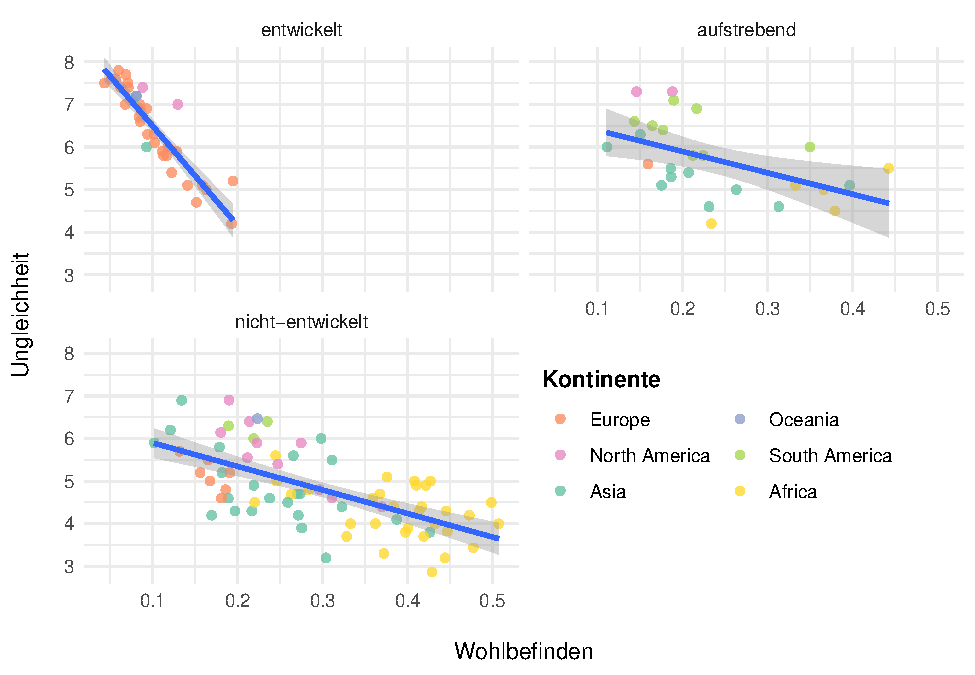
\includegraphics{PDFoutputsamples_files/figure-latex/unnamed-chunk-4-1.pdf}

\newpage

\hypertarget{scatter}{%
\subsubsection{Scatter}\label{scatter}}

Lorem ipsum dolor sit amet, consetetur sadipscing elitr, sed diam nonumy
eirmod tempor invidunt ut labore et dolore magna aliquyam erat, sed diam
voluptua. At vero eos et accusam et justo duo dolores et ea rebum. Stet
clita kasd gubergren, no sea takimata sanctus est Lorem ipsum dolor sit
amet.

Lorem ipsum dolor sit amet, consetetur sadipscing elitr, sed diam nonumy
eirmod tempor invidunt ut labore et dolore magna aliquyam erat, sed diam
voluptua. At vero eos et accusam et justo duo dolores et ea rebum. Stet
clita kasd gubergren, no sea takimata sanctus est Lorem ipsum dolor sit
amet.

\twocolumn

Lorem ipsum dolor sit amet, consetetur sadipscing elitr, sed diam nonumy
eirmod tempor invidunt ut labore et dolore magna aliquyam erat, sed diam
voluptua. At vero eos et accusam et justo duo dolores et ea rebum. Stet
clita kasd gubergren, no sea takimata sanctus est Lorem ipsum dolor sit
amet. Lorem ipsum dolor sit amet, consetetur sadipscing elitr, sed diam
nonumy eirmod tempor invidunt ut labore et dolore magna aliquyam erat,
sed diam voluptua. At vero eos et accusam et justo duo dolores et ea
rebum. Stet clita kasd gubergren, no sea takimata sanctus est Lorem
ipsum dolor sit amet.

\begin{verbatim}
## `geom_smooth()` using formula 'y ~ x'
\end{verbatim}

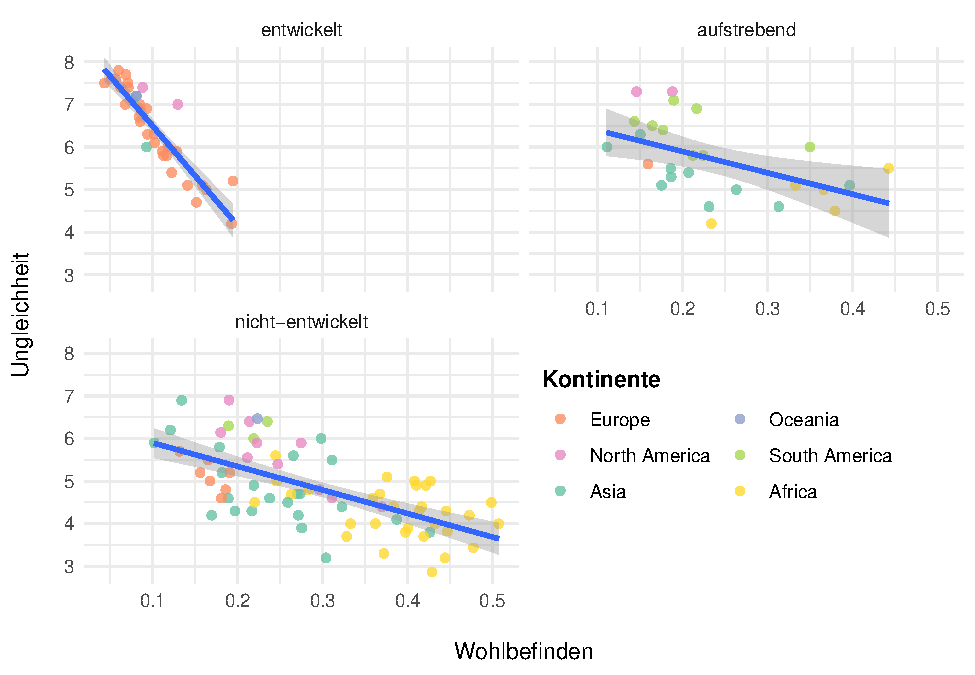
\includegraphics{PDFoutputsamples_files/figure-latex/unnamed-chunk-6-1.pdf}

\newpage
\onecolumn

\hypertarget{kableextra}{%
\subsubsection{kableExtra}\label{kableextra}}

\begin{Shaded}
\begin{Highlighting}[]
\NormalTok{kableData <-}\StringTok{ }\NormalTok{WorldData }\OperatorTok\StringTok{ }
\StringTok{  }\KeywordTok{select}\NormalTok{(}
\NormalTok{    continent,}
\NormalTok{    pop_est_dens,}
\NormalTok{    gdp_cap_est,}
\NormalTok{    life_exp,}
\NormalTok{    well_being,}
\NormalTok{    inequality,}
\NormalTok{    HPI) }\OperatorTok\StringTok{ }
\StringTok{  }\KeywordTok{group_by}\NormalTok{(continent) }\OperatorTok\StringTok{ }
\StringTok{  }\KeywordTok{summarise}\NormalTok{(}
    \KeywordTok{across}\NormalTok{(}
\NormalTok{      pop_est_dens}\OperatorTok{:}\NormalTok{HPI, }
      \OperatorTok{~}\KeywordTok{round}\NormalTok{(}
        \KeywordTok{mean}\NormalTok{(., }\DataTypeTok{na.rm =} \OtherTok{TRUE}\NormalTok{)}
\NormalTok{        ,}\DecValTok{1}\NormalTok{))) }\OperatorTok\StringTok{ }
\StringTok{  }\KeywordTok{filter}\NormalTok{(}\OperatorTok{!}\KeywordTok{is.na}\NormalTok{(well_being)) }
\end{Highlighting}
\end{Shaded}

\begin{verbatim}
## `summarise()` ungrouping output (override with `.groups` argument)
\end{verbatim}

\begin{Shaded}
\begin{Highlighting}[]
\NormalTok{  kableExtra}\OperatorTok{::}\KeywordTok{kbl}\NormalTok{(kableData,}
    \DataTypeTok{col.names =} \KeywordTok{c}\NormalTok{(}
      \StringTok{"Kontinent"}\NormalTok{,}
      \StringTok{"Bevölkerungsdichte"}\NormalTok{,}
      \StringTok{"BIP (pro Kopf)"}\NormalTok{,}
      \StringTok{"Lebenserwartung"}\NormalTok{,}
      \StringTok{"Wohlbefinden"}\NormalTok{,}
      \StringTok{"Ungleichheit"}\NormalTok{,}
      \StringTok{"Happy Planet"}\NormalTok{),}
    \DataTypeTok{booktabs =}\NormalTok{ T) }\OperatorTok\StringTok{ }
\StringTok{  }\NormalTok{kableExtra}\OperatorTok{::}\KeywordTok{add_header_above}\NormalTok{(}\KeywordTok{c}\NormalTok{(}
    \StringTok{" "}\NormalTok{ =}\StringTok{ }\DecValTok{4}\NormalTok{, }
    \StringTok{"Index"}\NormalTok{ =}\StringTok{ }\DecValTok{3}\NormalTok{)) }\OperatorTok\StringTok{ }
\StringTok{  }\NormalTok{kableExtra}\OperatorTok{::}\KeywordTok{kable_styling}\NormalTok{(}\DataTypeTok{latex_options =} \KeywordTok{c}\NormalTok{(}
    \StringTok{"striped"}\NormalTok{,}
    \StringTok{"scale_down"}\NormalTok{,}
    \StringTok{"reapeat_header"}\NormalTok{))}
\end{Highlighting}
\end{Shaded}

\begin{table}[H]
\centering
\resizebox{\linewidth}{!}{
\begin{tabular}[t]{lrrrrrr}
\toprule
\multicolumn{4}{c}{ } & \multicolumn{3}{c}{Index} \\
\cmidrule(l{3pt}r{3pt}){5-7}
Kontinent & Bevölkerungsdichte & BIP (pro Kopf) & Lebenserwartung & Wohlbefinden & Ungleichheit & Happy Planet\\
\midrule
\cellcolor{gray!6}{Africa} & \cellcolor{gray!6}{60.4} & \cellcolor{gray!6}{3391.9} & \cellcolor{gray!6}{59.8} & \cellcolor{gray!6}{4.4} & \cellcolor{gray!6}{0.4} & \cellcolor{gray!6}{19.9}\\
Asia & 176.0 & 13605.7 & 71.7 & 5.1 & 0.2 & 27.9\\
\cellcolor{gray!6}{Europe} & \cellcolor{gray!6}{114.6} & \cellcolor{gray!6}{25960.5} & \cellcolor{gray!6}{77.9} & \cellcolor{gray!6}{6.1} & \cellcolor{gray!6}{0.1} & \cellcolor{gray!6}{27.2}\\
North America & 136.3 & 14725.4 & 73.9 & 6.1 & 0.2 & 32.2\\
\cellcolor{gray!6}{Oceania} & \cellcolor{gray!6}{19.4} & \cellcolor{gray!6}{13074.2} & \cellcolor{gray!6}{78.3} & \cellcolor{gray!6}{7.0} & \cellcolor{gray!6}{0.1} & \cellcolor{gray!6}{31.0}\\
\addlinespace
South America & 20.6 & 11045.6 & 74.2 & 6.3 & 0.2 & 32.3\\
\bottomrule
\end{tabular}}
\end{table}

\end{document}
